% Options for packages loaded elsewhere
\PassOptionsToPackage{unicode}{hyperref}
\PassOptionsToPackage{hyphens}{url}
%
\documentclass[
]{article}
\usepackage{amsmath,amssymb}
\usepackage{iftex}
\ifPDFTeX
  \usepackage[T1]{fontenc}
  \usepackage[utf8]{inputenc}
  \usepackage{textcomp} % provide euro and other symbols
\else % if luatex or xetex
  \usepackage{unicode-math} % this also loads fontspec
  \defaultfontfeatures{Scale=MatchLowercase}
  \defaultfontfeatures[\rmfamily]{Ligatures=TeX,Scale=1}
\fi
\usepackage{lmodern}
\ifPDFTeX\else
  % xetex/luatex font selection
\fi
% Use upquote if available, for straight quotes in verbatim environments
\IfFileExists{upquote.sty}{\usepackage{upquote}}{}
\IfFileExists{microtype.sty}{% use microtype if available
  \usepackage[]{microtype}
  \UseMicrotypeSet[protrusion]{basicmath} % disable protrusion for tt fonts
}{}
\makeatletter
\@ifundefined{KOMAClassName}{% if non-KOMA class
  \IfFileExists{parskip.sty}{%
    \usepackage{parskip}
  }{% else
    \setlength{\parindent}{0pt}
    \setlength{\parskip}{6pt plus 2pt minus 1pt}}
}{% if KOMA class
  \KOMAoptions{parskip=half}}
\makeatother
\usepackage{xcolor}
\usepackage[margin=1in]{geometry}
\usepackage{color}
\usepackage{fancyvrb}
\newcommand{\VerbBar}{|}
\newcommand{\VERB}{\Verb[commandchars=\\\{\}]}
\DefineVerbatimEnvironment{Highlighting}{Verbatim}{commandchars=\\\{\}}
% Add ',fontsize=\small' for more characters per line
\usepackage{framed}
\definecolor{shadecolor}{RGB}{248,248,248}
\newenvironment{Shaded}{\begin{snugshade}}{\end{snugshade}}
\newcommand{\AlertTok}[1]{\textcolor[rgb]{0.94,0.16,0.16}{#1}}
\newcommand{\AnnotationTok}[1]{\textcolor[rgb]{0.56,0.35,0.01}{\textbf{\textit{#1}}}}
\newcommand{\AttributeTok}[1]{\textcolor[rgb]{0.13,0.29,0.53}{#1}}
\newcommand{\BaseNTok}[1]{\textcolor[rgb]{0.00,0.00,0.81}{#1}}
\newcommand{\BuiltInTok}[1]{#1}
\newcommand{\CharTok}[1]{\textcolor[rgb]{0.31,0.60,0.02}{#1}}
\newcommand{\CommentTok}[1]{\textcolor[rgb]{0.56,0.35,0.01}{\textit{#1}}}
\newcommand{\CommentVarTok}[1]{\textcolor[rgb]{0.56,0.35,0.01}{\textbf{\textit{#1}}}}
\newcommand{\ConstantTok}[1]{\textcolor[rgb]{0.56,0.35,0.01}{#1}}
\newcommand{\ControlFlowTok}[1]{\textcolor[rgb]{0.13,0.29,0.53}{\textbf{#1}}}
\newcommand{\DataTypeTok}[1]{\textcolor[rgb]{0.13,0.29,0.53}{#1}}
\newcommand{\DecValTok}[1]{\textcolor[rgb]{0.00,0.00,0.81}{#1}}
\newcommand{\DocumentationTok}[1]{\textcolor[rgb]{0.56,0.35,0.01}{\textbf{\textit{#1}}}}
\newcommand{\ErrorTok}[1]{\textcolor[rgb]{0.64,0.00,0.00}{\textbf{#1}}}
\newcommand{\ExtensionTok}[1]{#1}
\newcommand{\FloatTok}[1]{\textcolor[rgb]{0.00,0.00,0.81}{#1}}
\newcommand{\FunctionTok}[1]{\textcolor[rgb]{0.13,0.29,0.53}{\textbf{#1}}}
\newcommand{\ImportTok}[1]{#1}
\newcommand{\InformationTok}[1]{\textcolor[rgb]{0.56,0.35,0.01}{\textbf{\textit{#1}}}}
\newcommand{\KeywordTok}[1]{\textcolor[rgb]{0.13,0.29,0.53}{\textbf{#1}}}
\newcommand{\NormalTok}[1]{#1}
\newcommand{\OperatorTok}[1]{\textcolor[rgb]{0.81,0.36,0.00}{\textbf{#1}}}
\newcommand{\OtherTok}[1]{\textcolor[rgb]{0.56,0.35,0.01}{#1}}
\newcommand{\PreprocessorTok}[1]{\textcolor[rgb]{0.56,0.35,0.01}{\textit{#1}}}
\newcommand{\RegionMarkerTok}[1]{#1}
\newcommand{\SpecialCharTok}[1]{\textcolor[rgb]{0.81,0.36,0.00}{\textbf{#1}}}
\newcommand{\SpecialStringTok}[1]{\textcolor[rgb]{0.31,0.60,0.02}{#1}}
\newcommand{\StringTok}[1]{\textcolor[rgb]{0.31,0.60,0.02}{#1}}
\newcommand{\VariableTok}[1]{\textcolor[rgb]{0.00,0.00,0.00}{#1}}
\newcommand{\VerbatimStringTok}[1]{\textcolor[rgb]{0.31,0.60,0.02}{#1}}
\newcommand{\WarningTok}[1]{\textcolor[rgb]{0.56,0.35,0.01}{\textbf{\textit{#1}}}}
\usepackage{graphicx}
\makeatletter
\newsavebox\pandoc@box
\newcommand*\pandocbounded[1]{% scales image to fit in text height/width
  \sbox\pandoc@box{#1}%
  \Gscale@div\@tempa{\textheight}{\dimexpr\ht\pandoc@box+\dp\pandoc@box\relax}%
  \Gscale@div\@tempb{\linewidth}{\wd\pandoc@box}%
  \ifdim\@tempb\p@<\@tempa\p@\let\@tempa\@tempb\fi% select the smaller of both
  \ifdim\@tempa\p@<\p@\scalebox{\@tempa}{\usebox\pandoc@box}%
  \else\usebox{\pandoc@box}%
  \fi%
}
% Set default figure placement to htbp
\def\fps@figure{htbp}
\makeatother
\setlength{\emergencystretch}{3em} % prevent overfull lines
\providecommand{\tightlist}{%
  \setlength{\itemsep}{0pt}\setlength{\parskip}{0pt}}
\setcounter{secnumdepth}{-\maxdimen} % remove section numbering
\usepackage{bookmark}
\IfFileExists{xurl.sty}{\usepackage{xurl}}{} % add URL line breaks if available
\urlstyle{same}
\hypersetup{
  pdftitle={EDA\_Covid\_19\_Prevention\_National\_04},
  pdfauthor={Group K},
  hidelinks,
  pdfcreator={LaTeX via pandoc}}

\title{EDA\_Covid\_19\_Prevention\_National\_04}
\author{Group K}
\date{2025-09-09}

\begin{document}
\maketitle

\begin{Shaded}
\begin{Highlighting}[]
\FunctionTok{library}\NormalTok{(readr)}
\FunctionTok{library}\NormalTok{(ggplot2)}
\FunctionTok{library}\NormalTok{(dplyr)}
\FunctionTok{library}\NormalTok{(here)}

\FunctionTok{getwd}\NormalTok{()}
\end{Highlighting}
\end{Shaded}

\begin{verbatim}
## [1] "C:/Users/Tshiamo/OneDrive/Documents/Belgium Campus iTversity/BComp 2025/BIN381/Project/BIN381-Project/scripts"
\end{verbatim}

\begin{Shaded}
\begin{Highlighting}[]
\FunctionTok{list.files}\NormalTok{(}\StringTok{"data/raw\_data"}\NormalTok{)}
\end{Highlighting}
\end{Shaded}

\begin{verbatim}
## character(0)
\end{verbatim}

\section{Load data and show the
structure}\label{load-data-and-show-the-structure}

\begin{Shaded}
\begin{Highlighting}[]
\NormalTok{cop\_df }\OtherTok{\textless{}{-}} \FunctionTok{read\_csv}\NormalTok{(}\FunctionTok{here}\NormalTok{(}\StringTok{"raw\_data"}\NormalTok{, }\StringTok{"covid{-}19{-}prevention\_national\_zaf.csv"}\NormalTok{))}
\end{Highlighting}
\end{Shaded}

\begin{verbatim}
## Rows: 35 Columns: 29
## -- Column specification --------------------------------------------------------
## Delimiter: ","
## chr (17): ISO3, DataId, Indicator, Value, Precision, DHS_CountryCode, Countr...
## dbl  (8): IndicatorOrder, CharacteristicId, CharacteristicOrder, IsTotal, Is...
## lgl  (4): RegionId, CILow, CIHigh, LevelRank
## 
## i Use `spec()` to retrieve the full column specification for this data.
## i Specify the column types or set `show_col_types = FALSE` to quiet this message.
\end{verbatim}

\#Dislay the first and last 10 rows

\begin{Shaded}
\begin{Highlighting}[]
\FunctionTok{head}\NormalTok{(cop\_df, }\DecValTok{10}\NormalTok{)}
\end{Highlighting}
\end{Shaded}

\begin{verbatim}
## # A tibble: 10 x 29
##    ISO3  DataId Indicator Value Precision DHS_CountryCode CountryName SurveyYear
##    <chr> <chr>  <chr>     <chr> <chr>     <chr>           <chr>       <chr>     
##  1 #cou~ #meta~ #indicat~ #ind~ #indicat~ <NA>            #country+n~ #date+year
##  2 ZAF   795844 Populati~ 83.5  1         ZA              South Afri~ 1998      
##  3 ZAF   795750 Populati~ 36    1         ZA              South Afri~ 1998      
##  4 ZAF   795755 Populati~ 23.1  1         ZA              South Afri~ 1998      
##  5 ZAF   795740 Populati~ 19.3  1         ZA              South Afri~ 1998      
##  6 ZAF   795744 Populati~ 60.3  1         ZA              South Afri~ 1998      
##  7 ZAF   795754 Populati~ 80.2  1         ZA              South Afri~ 1998      
##  8 ZAF   795749 Populati~ 3.3   1         ZA              South Afri~ 1998      
##  9 ZAF   795743 Populati~ 8.4   1         ZA              South Afri~ 1998      
## 10 ZAF   795102 Populati~ 46.4  1         ZA              South Afri~ 1998      
## # i 21 more variables: SurveyId <chr>, IndicatorId <chr>, IndicatorOrder <dbl>,
## #   IndicatorType <chr>, CharacteristicId <dbl>, CharacteristicOrder <dbl>,
## #   CharacteristicCategory <chr>, CharacteristicLabel <chr>,
## #   ByVariableId <chr>, ByVariableLabel <chr>, IsTotal <dbl>,
## #   IsPreferred <dbl>, SDRID <chr>, RegionId <lgl>, SurveyYearLabel <dbl>,
## #   SurveyType <chr>, DenominatorWeighted <dbl>, DenominatorUnweighted <dbl>,
## #   CILow <lgl>, CIHigh <lgl>, LevelRank <lgl>
\end{verbatim}

\begin{Shaded}
\begin{Highlighting}[]
\FunctionTok{tail}\NormalTok{(cop\_df, }\DecValTok{10}\NormalTok{)}
\end{Highlighting}
\end{Shaded}

\begin{verbatim}
## # A tibble: 10 x 29
##    ISO3  DataId Indicator Value Precision DHS_CountryCode CountryName SurveyYear
##    <chr> <chr>  <chr>     <chr> <chr>     <chr>           <chr>       <chr>     
##  1 ZAF   456204 Populati~ 1.7   1         ZA              South Afri~ 2016      
##  2 ZAF   456210 Populati~ 2.2   1         ZA              South Afri~ 2016      
##  3 ZAF   456218 Populati~ 81.1  1         ZA              South Afri~ 2016      
##  4 ZAF   456217 Populati~ 15    1         ZA              South Afri~ 2016      
##  5 ZAF   622821 Populati~ 86.1  1         ZA              South Afri~ 2016      
##  6 ZAF   30013  Populati~ 46    1         ZA              South Afri~ 2016      
##  7 ZAF   30014  Populati~ 46.5  1         ZA              South Afri~ 2016      
##  8 ZAF   197801 Househol~ 35.1  1         ZA              South Afri~ 2016      
##  9 ZAF   197811 Mean num~ 1.5   1         ZA              South Afri~ 2016      
## 10 ZAF   618821 Mean num~ 3.4   1         ZA              South Afri~ 2016      
## # i 21 more variables: SurveyId <chr>, IndicatorId <chr>, IndicatorOrder <dbl>,
## #   IndicatorType <chr>, CharacteristicId <dbl>, CharacteristicOrder <dbl>,
## #   CharacteristicCategory <chr>, CharacteristicLabel <chr>,
## #   ByVariableId <chr>, ByVariableLabel <chr>, IsTotal <dbl>,
## #   IsPreferred <dbl>, SDRID <chr>, RegionId <lgl>, SurveyYearLabel <dbl>,
## #   SurveyType <chr>, DenominatorWeighted <dbl>, DenominatorUnweighted <dbl>,
## #   CILow <lgl>, CIHigh <lgl>, LevelRank <lgl>
\end{verbatim}

\#Dimenison of the data

\begin{Shaded}
\begin{Highlighting}[]
\FunctionTok{dim}\NormalTok{(cop\_df)}
\end{Highlighting}
\end{Shaded}

\begin{verbatim}
## [1] 35 29
\end{verbatim}

\#Provide a summary of the datset

\begin{Shaded}
\begin{Highlighting}[]
\FunctionTok{summary}\NormalTok{(cop\_df)}
\end{Highlighting}
\end{Shaded}

\begin{verbatim}
##      ISO3              DataId           Indicator            Value          
##  Length:35          Length:35          Length:35          Length:35         
##  Class :character   Class :character   Class :character   Class :character  
##  Mode  :character   Mode  :character   Mode  :character   Mode  :character  
##                                                                             
##                                                                             
##                                                                             
##                                                                             
##   Precision         DHS_CountryCode    CountryName         SurveyYear       
##  Length:35          Length:35          Length:35          Length:35         
##  Class :character   Class :character   Class :character   Class :character  
##  Mode  :character   Mode  :character   Mode  :character   Mode  :character  
##                                                                             
##                                                                             
##                                                                             
##                                                                             
##    SurveyId         IndicatorId        IndicatorOrder      IndicatorType     
##  Length:35          Length:35          Min.   :250162010   Length:35         
##  Class :character   Class :character   1st Qu.:250162190   Class :character  
##  Mode  :character   Mode  :character   Median :250252010   Mode  :character  
##                                        Mean   :252040162                     
##                                        3rd Qu.:250292085                     
##                                        Max.   :260831120                     
##                                        NA's   :1                             
##  CharacteristicId CharacteristicOrder CharacteristicCategory
##  Min.   :1000     Min.   :0           Length:35             
##  1st Qu.:1000     1st Qu.:0           Class :character      
##  Median :1000     Median :0           Mode  :character      
##  Mean   :1000     Mean   :0                                 
##  3rd Qu.:1000     3rd Qu.:0                                 
##  Max.   :1000     Max.   :0                                 
##  NA's   :1        NA's   :1                                 
##  CharacteristicLabel ByVariableId       ByVariableLabel       IsTotal 
##  Length:35           Length:35          Length:35          Min.   :1  
##  Class :character    Class :character   Class :character   1st Qu.:1  
##  Mode  :character    Mode  :character   Mode  :character   Median :1  
##                                                            Mean   :1  
##                                                            3rd Qu.:1  
##                                                            Max.   :1  
##                                                            NA's   :1  
##   IsPreferred    SDRID           RegionId       SurveyYearLabel
##  Min.   :1    Length:35          Mode:logical   Min.   :1998   
##  1st Qu.:1    Class :character   NA's:35        1st Qu.:1998   
##  Median :1    Mode  :character                  Median :2016   
##  Mean   :1                                      Mean   :2009   
##  3rd Qu.:1                                      3rd Qu.:2016   
##  Max.   :1                                      Max.   :2016   
##  NA's   :1                                      NA's   :1      
##   SurveyType        DenominatorWeighted DenominatorUnweighted  CILow        
##  Length:35          Min.   :11066       Min.   :11066         Mode:logical  
##  Class :character   1st Qu.:37205       1st Qu.:37925         NA's:35       
##  Mode  :character   Median :37205       Median :37925                       
##                     Mean   :38815       Mean   :39353                       
##                     3rd Qu.:52007       3rd Qu.:52465                       
##                     Max.   :52007       Max.   :52465                       
##                     NA's   :3           NA's   :3                           
##   CIHigh        LevelRank     
##  Mode:logical   Mode:logical  
##  NA's:35        NA's:35       
##                               
##                               
##                               
##                               
## 
\end{verbatim}

\#Convert Value to a numeric

\begin{Shaded}
\begin{Highlighting}[]
\NormalTok{cop\_df}\SpecialCharTok{$}\NormalTok{Value }\OtherTok{\textless{}{-}} \FunctionTok{as.numeric}\NormalTok{(cop\_df}\SpecialCharTok{$}\NormalTok{Value)}
\end{Highlighting}
\end{Shaded}

\begin{verbatim}
## Warning: NAs introduced by coercion
\end{verbatim}

\#Find duplicated values

\begin{Shaded}
\begin{Highlighting}[]
\FunctionTok{sum}\NormalTok{(}\FunctionTok{duplicated}\NormalTok{(cop\_df))}
\end{Highlighting}
\end{Shaded}

\begin{verbatim}
## [1] 0
\end{verbatim}

\#Inspect columns for missing/empty data as values and pecentages
respectively

\begin{Shaded}
\begin{Highlighting}[]
\FunctionTok{colSums}\NormalTok{(}\FunctionTok{is.na}\NormalTok{(cop\_df))}
\end{Highlighting}
\end{Shaded}

\begin{verbatim}
##                   ISO3                 DataId              Indicator 
##                      0                      0                      0 
##                  Value              Precision        DHS_CountryCode 
##                      1                      0                      1 
##            CountryName             SurveyYear               SurveyId 
##                      0                      0                      0 
##            IndicatorId         IndicatorOrder          IndicatorType 
##                      0                      1                      1 
##       CharacteristicId    CharacteristicOrder CharacteristicCategory 
##                      1                      1                      1 
##    CharacteristicLabel           ByVariableId        ByVariableLabel 
##                      1                      0                     34 
##                IsTotal            IsPreferred                  SDRID 
##                      1                      1                      1 
##               RegionId        SurveyYearLabel             SurveyType 
##                     35                      1                      1 
##    DenominatorWeighted  DenominatorUnweighted                  CILow 
##                      3                      3                     35 
##                 CIHigh              LevelRank 
##                     35                     35
\end{verbatim}

\begin{Shaded}
\begin{Highlighting}[]
\FunctionTok{round}\NormalTok{(}\FunctionTok{colMeans}\NormalTok{(}\FunctionTok{is.na}\NormalTok{(cop\_df)) }\SpecialCharTok{*} \DecValTok{100}\NormalTok{, }\DecValTok{2}\NormalTok{)}
\end{Highlighting}
\end{Shaded}

\begin{verbatim}
##                   ISO3                 DataId              Indicator 
##                   0.00                   0.00                   0.00 
##                  Value              Precision        DHS_CountryCode 
##                   2.86                   0.00                   2.86 
##            CountryName             SurveyYear               SurveyId 
##                   0.00                   0.00                   0.00 
##            IndicatorId         IndicatorOrder          IndicatorType 
##                   0.00                   2.86                   2.86 
##       CharacteristicId    CharacteristicOrder CharacteristicCategory 
##                   2.86                   2.86                   2.86 
##    CharacteristicLabel           ByVariableId        ByVariableLabel 
##                   2.86                   0.00                  97.14 
##                IsTotal            IsPreferred                  SDRID 
##                   2.86                   2.86                   2.86 
##               RegionId        SurveyYearLabel             SurveyType 
##                 100.00                   2.86                   2.86 
##    DenominatorWeighted  DenominatorUnweighted                  CILow 
##                   8.57                   8.57                 100.00 
##                 CIHigh              LevelRank 
##                 100.00                 100.00
\end{verbatim}

\section{Check for unique values}\label{check-for-unique-values}

\begin{Shaded}
\begin{Highlighting}[]
\FunctionTok{sapply}\NormalTok{(cop\_df, }\ControlFlowTok{function}\NormalTok{(x) }\FunctionTok{length}\NormalTok{(}\FunctionTok{unique}\NormalTok{(x)))}
\end{Highlighting}
\end{Shaded}

\begin{verbatim}
##                   ISO3                 DataId              Indicator 
##                      2                     35                     21 
##                  Value              Precision        DHS_CountryCode 
##                     35                      3                      2 
##            CountryName             SurveyYear               SurveyId 
##                      2                      3                      3 
##            IndicatorId         IndicatorOrder          IndicatorType 
##                     21                     21                      2 
##       CharacteristicId    CharacteristicOrder CharacteristicCategory 
##                      2                      2                      2 
##    CharacteristicLabel           ByVariableId        ByVariableLabel 
##                      2                      2                      2 
##                IsTotal            IsPreferred                  SDRID 
##                      2                      2                     21 
##               RegionId        SurveyYearLabel             SurveyType 
##                      1                      3                      2 
##    DenominatorWeighted  DenominatorUnweighted                  CILow 
##                      9                      9                      1 
##                 CIHigh              LevelRank 
##                      1                      1
\end{verbatim}

\#Plots

\begin{Shaded}
\begin{Highlighting}[]
\CommentTok{\#Histogram of Values}

\FunctionTok{ggplot}\NormalTok{(cop\_df, }\FunctionTok{aes}\NormalTok{(}\AttributeTok{x =}\NormalTok{ Value)) }\SpecialCharTok{+}
\FunctionTok{geom\_histogram}\NormalTok{(}\AttributeTok{bins =} \DecValTok{30}\NormalTok{, }\AttributeTok{fill =} \StringTok{"skyblue"}\NormalTok{, }\AttributeTok{color =} \StringTok{"black"}\NormalTok{) }\SpecialCharTok{+}
  \FunctionTok{labs}\NormalTok{(}\AttributeTok{title =} \StringTok{"Distribution of Indicator Values"}\NormalTok{)}
\end{Highlighting}
\end{Shaded}

\begin{verbatim}
## Warning: Removed 1 row containing non-finite outside the scale range
## (`stat_bin()`).
\end{verbatim}

\pandocbounded{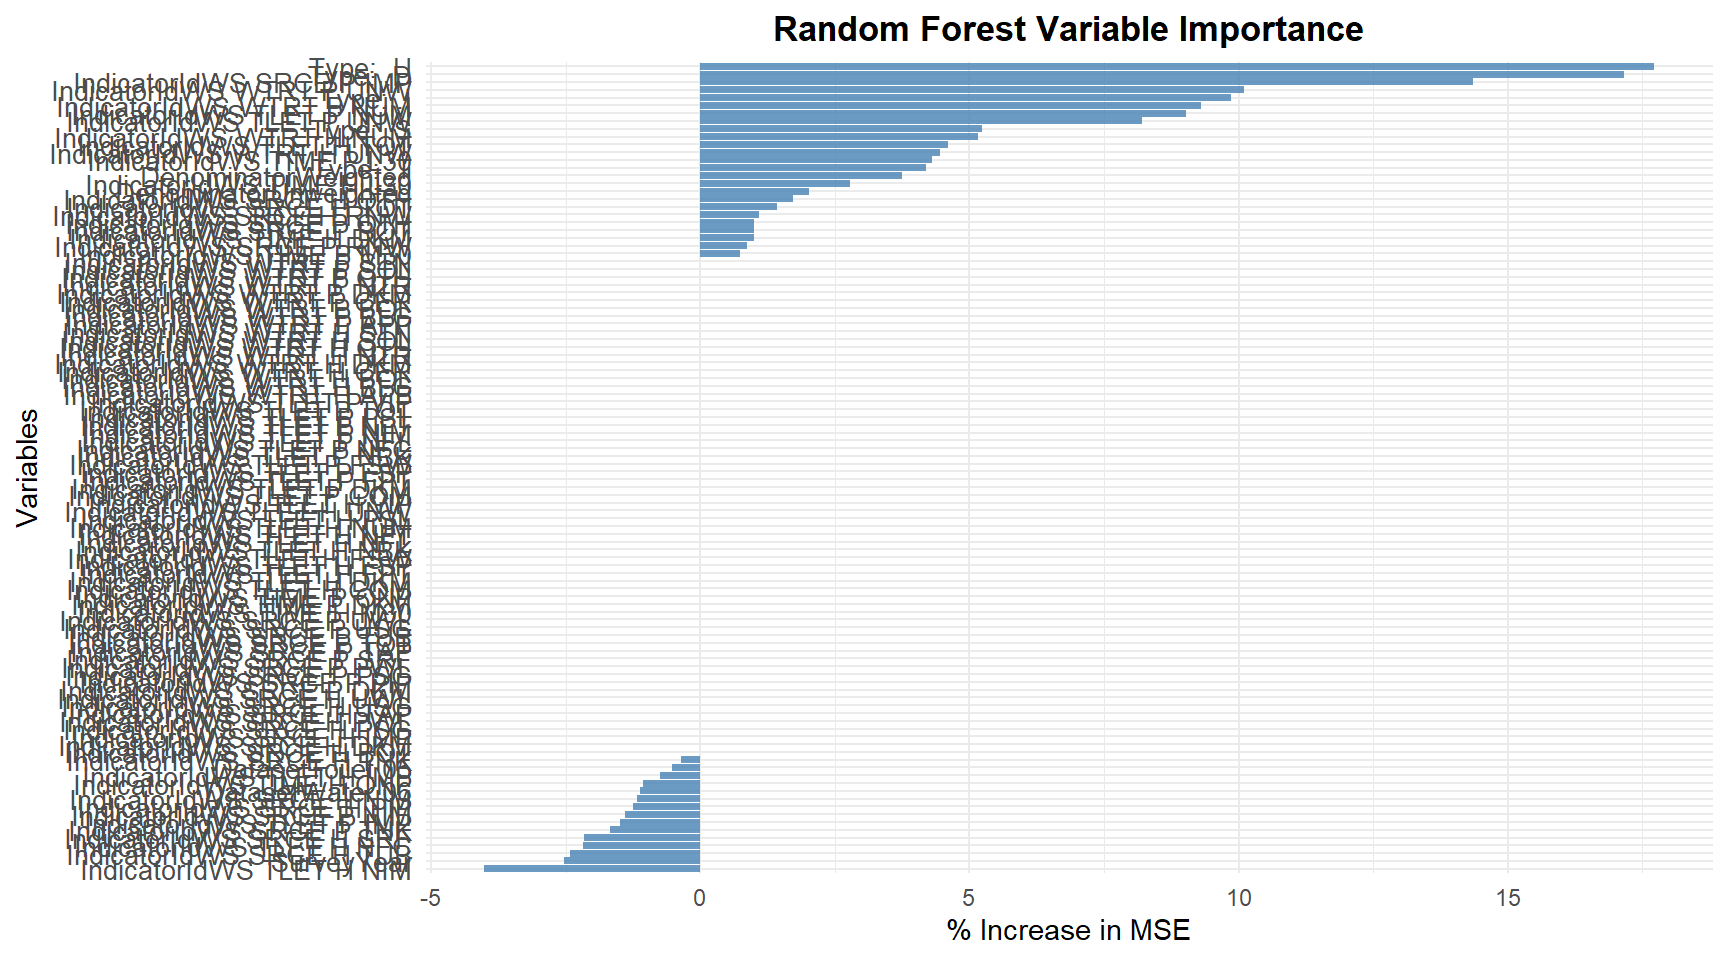
\includegraphics[keepaspectratio]{EDA_Covid_19_National_04_files/figure-latex/unnamed-chunk-9-1.pdf}}

\begin{Shaded}
\begin{Highlighting}[]
\FunctionTok{ggsave}\NormalTok{(}\StringTok{"../outputs/visuals/covid\_rate\_histo.png"}\NormalTok{, }\AttributeTok{width =} \DecValTok{6}\NormalTok{, }\AttributeTok{height =} \DecValTok{4}\NormalTok{)}
\end{Highlighting}
\end{Shaded}

\begin{verbatim}
## Warning: Removed 1 row containing non-finite outside the scale range
## (`stat_bin()`).
\end{verbatim}

\begin{Shaded}
\begin{Highlighting}[]
\CommentTok{\#Outliers}
\FunctionTok{boxplot}\NormalTok{(cop\_df}\SpecialCharTok{$}\NormalTok{Value, }\AttributeTok{main =} \StringTok{"Outlier check for Values"}\NormalTok{)}
\end{Highlighting}
\end{Shaded}

\pandocbounded{\includegraphics[keepaspectratio]{EDA_Covid_19_National_04_files/figure-latex/unnamed-chunk-9-2.pdf}}

\end{document}
